%==============================================================================
% locality-performance.tex
%==============================================================================

\chapter{Performance Evaluation}
\label{chap:locality-performance}

The performance results in this chapter are obtained on an Intel
Nehalem system with two processors and eight cores, running Ubuntu
9.04 64-bit with kernel 2.6.29 and Sun Hotspot JDK 1.6.0\_20 (Appendix
\ref{sec:experimental-setup-mafushi}). The JVM is invoked with the
following parameters:

\begin{lstlisting}[style=Listing]
  -server -Xmx4096M -Xms4096M -Xss8M -XX:+UseNUMA
\end{lstlisting}

It is important that our new scheduler implementation does not affect
the performance of existing locality-ignorant intervals
programs. Thus, we run the locality-ignorant JGF benchmarks (Appendix
\ref{chap:benchmarks}) with our new scheduler implementation. As
Figure \ref{fig:locality-evaluation-jgf} shows, the performance of
locality-ignorant JGF benchmarks on the locality-aware intervals
scheduler is comparable to the original implementation.

\begin{figure}[!ht]
  \centering
  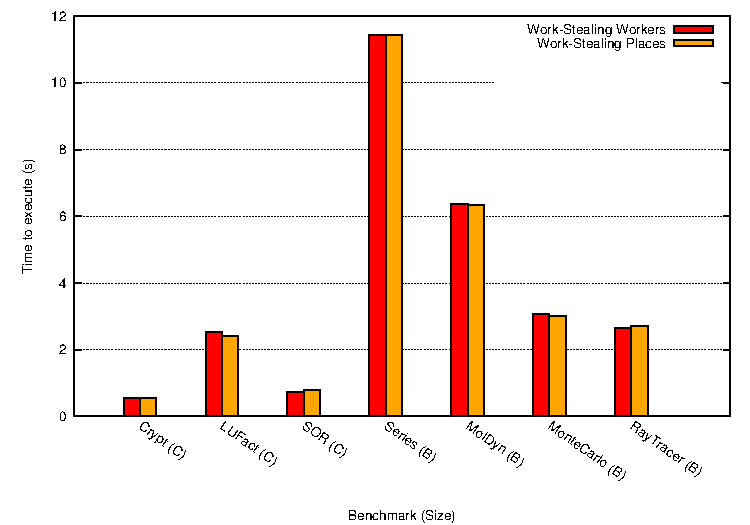
\includegraphics[width=0.6\linewidth]{locality-evaluation/mafushi-jgf}
  \caption[Locality-ignorant JGF benchmarks running on locality-aware
  scheduler]{Locality-ignorant JGF benchmarks using the locality-aware
    scheduler on our Intel Nehalem (Appendix
    \ref{sec:experimental-setup-mafushi}) test machine}
  \label{fig:locality-evaluation-jgf}
\end{figure}

The rest of this chapter evaluates the performance of the new
intervals scheduler on three different locality-aware benchmarks. To
reduce the impact of JVM overheads in the evaluation, the execution
time reported is the average of the three best from 10 benchmark
iterations.

\section{Cache-Stress Test}
\label{sec:locality-performance-cache-stress-test}

\begin{table}[htb]
  \centering
  \begin{tabular}{ln{2}{3}n{1}{2}}
    \toprule
    & {Runtime (in seconds)} & {Speedup (over sequential)} \\\midrule
    \emph{Best Locality} & 3.596 & 7.11 \\
    \emph{Ignorant Locality} & 4.038 & 6.33 \\
    \emph{Random Locality} & 4.030 & 6.35 \\
    \emph{Worst Locality} & 3.982 & 6.42 \\
    \emph{Sequential Implementation}\hspace{0.5cm} & 25.571 & 1 \\\bottomrule
  \end{tabular}
  \caption{\emph{Cache Stress Test} execution times and speedups over sequential implementation}
  \label{tab:locality-performance-cache-stress-test}
\end{table}

\begin{figure}[!ht]
  \centering
  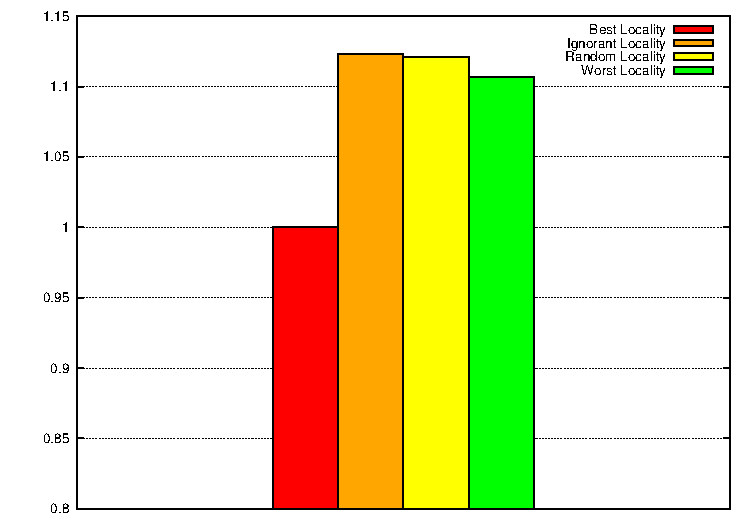
\includegraphics[width=0.7\linewidth]{locality-performance/cache-stress-test}
  \caption{\emph{Cache Stress Test} with execution times normalized to
    \emph{best locality}}
  \label{fig:locality-performance-cache-stress-test}
\end{figure}

\todo{Describe benchmark ``Cache-Stress Test''}

\begin{table}[htb]
  \centering
  \begin{tabular}{ln{4}{0}n{4}{0}}
    \toprule
    & {L3 Cache Read Misses} & {L3 Cache Read Hits} \\\midrule
    \emph{Best Locality}\hspace{1cm} & 275 & 2335 \\
    \emph{Ignorant Locality} & 837 & 1568 \\
    \emph{Random Locality} & 854 & 1570 \\
    \emph{Worst Locality} & 837 & 1539 \\\bottomrule
  \end{tabular}
  \caption[\emph{Cache Stress Test} L3 cache read misses and hits]
  {\emph{Cache Stress Test} L3 cache read misses and hits (rounded to the nearest million)}
  \label{tab:locality-performance-cache-stress-test-cache-misses}
\end{table}

\begin{figure}[!ht]
  \centering
  \subfloat[L3 Cache Read Misses]{
    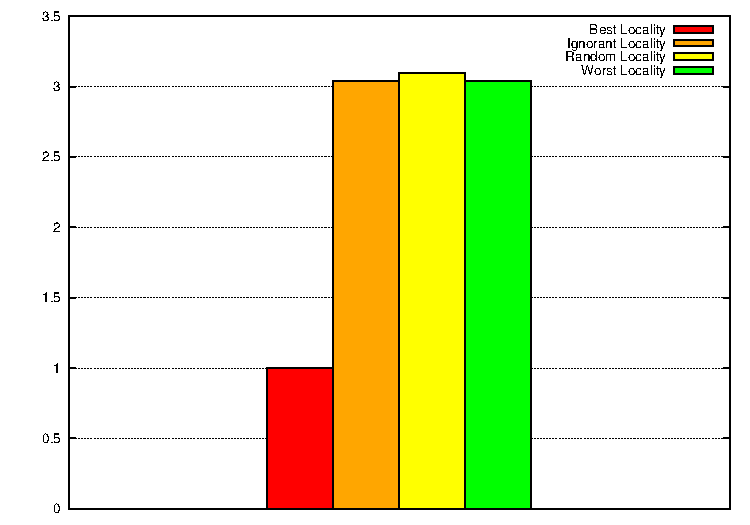
\includegraphics[width=0.5\linewidth]{locality-performance/cache-stress-test-cache-misses}
    \label{fig:locality-performance-cache-stress-test-cache-misses}
  }
  \subfloat[L3 Cache Read Hits]{
    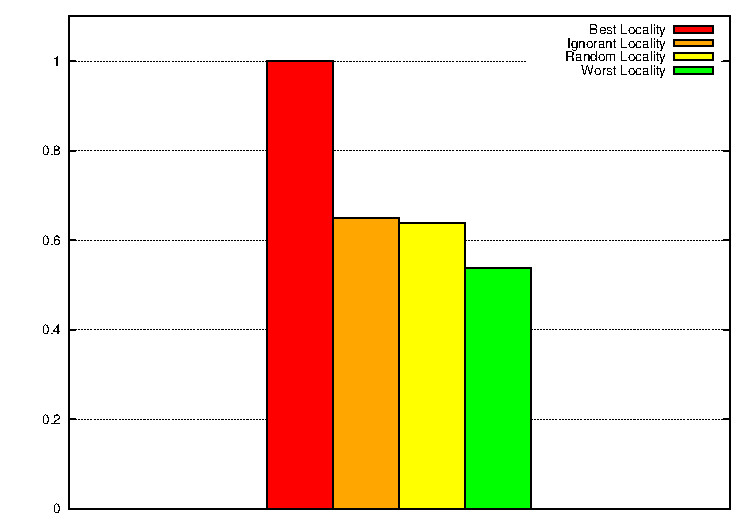
\includegraphics[width=0.5\linewidth]{locality-performance/cache-stress-test-cache-hits}
    \label{fig:locality-performance-cache-stress-test-cache-hits}
  }
  \caption{\emph{Cache Stress Test} with L3 cache read misses and hits
    normalized to \emph{best locality}}
  \label{fig:locality-performance-cache-stress-test-cache}
\end{figure}

\section{Merge Sort}
\label{sec:locality-performance-merge-sort}

\todo{Describe benchmark ``Merge Sort''}

\section{Block Matrix Multiplication}
\label{sec:locality-performance-block-matrix-multiplication}

\todo{Describe benchmark ``Block Matrix Multiplication''}

\section{References}

\subsection{Profiling}

\begin{itemize}
\item[\textbullet] Performance Counters on Linux - The New Tools
  \cite{Melo2009}
\item[\textbullet] Tuning programs with OProfile \cite{Cohen2004}
\item[\textbullet] Profiling with OProfile and Intel Core 2
  performance counters \cite{Nielsen2008}
\item[\textbullet] A Survey of Linux Measurement and Diagnostic Tools
  \cite{Rowand2009}
\item[\textbullet] Performance Characterization of SPEC CPU Benchmarks
  on Intel's Core Microarchitecture based processor \cite{Bird2007}
\item[\textbullet] What can performance counters do for memory
  subsystem analysis?  \cite{Eranian2008}
\item[\textbullet] Intel \textsuperscript{\textregistered} 64 and
  IA-32 Architectures Software Developer’s Manual - Volume 3B: System
  Programming Guide, Part 2 \cite{Intel2010}
\item[\textbullet] Intel \textsuperscript{\textregistered} 64 and
  IA-32 Architectures Optimization Reference Manual \cite{Intel2009}
\item[\textbullet] Can hardware performance counters be trusted?
  \cite{Weaver2008}
\item[\textbullet] Accuracy of performance counter measurements
  \cite{Zaparanuks2008}
\item[\textbullet] Performance Analysis Guide for Intel
  \textsuperscript{\textregistered} Core
  \textsuperscript{\texttrademark} i7 Processor and Intel
  \textsuperscript{\textregistered} Xeon
  \textsuperscript{\texttrademark} 5500 processors
  \cite{Levinthal2009}
\item[\textbullet] Using Intel \textsuperscript{\textregistered} VTune
  \textsuperscript{\texttrademark} Performance Analyzer to Optimize
  Software on Intel \textsuperscript{\textregistered} Core
  \textsuperscript{\texttrademark} i7 Processors \cite{Intel2009a}
\end{itemize}

\subsection{Multi-Threaded Algorithms}

\begin{itemize}
\item[\textbullet] Cache-oblivious algorithms \cite{Frigo1999}
\item[\textbullet] Cache-Oblivious Algorithms and Data Structures
  \cite{Demaine2002}
\item[\textbullet] Cache Oblivious Algorithms \cite{Kumar2003}
\item[\textbullet] The cache complexity of multithreaded cache
  oblivious algorithms \cite{Frigo2009}
\item[\textbullet] Divide-and-Conquer Algorithms \cite{Gurari2010}
\item[\textbullet] A minicourse on multithreaded programming
  \cite{Leiserson1998}
\item[\textbullet] Performance and Scalability Analysis of
  Parallelized Matrix Multiplication Using Shared Memory
  \cite{Dinkins2007}
\item[\textbullet] Designing efficient sorting algorithms for manycore
  GPUs \cite{Satish2009}
\item[\textbullet] A Tale of Two Algorithms: Multithreading Matrix
  Multiplication Overhead in Parallelism Choosing an Algorithm
  \cite{Steele2010}
\item[\textbullet] Algorithms for Multicore Computing
  \cite{Ramachandran2008}
\item[\textbullet] Fast recursive matrix multiplication for multi-core
  architectures \cite{Runger2010}
\item[\checkmark] Practical implementations of non-blocking
  synchronization primitives \cite{Moir1997}
\end{itemize}

\todo{Finish chapter ``Performance''}


%%% Local Variables: 
%%% mode: latex
%%% TeX-master: "thesis"
%%% End: 
